\documentclass{standalone}
\usepackage{tikz}
\usetikzlibrary{positioning}
\usetikzlibrary{fit}

\begin{document}

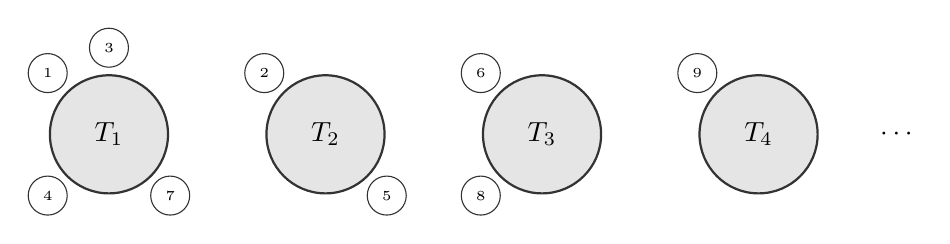
\begin{tikzpicture}
  \tikzstyle{table}=[circle, thick, draw = black!80, fill = black!10, minimum size = 15mm]
  \tikzstyle{customer}=[circle, thin, draw = black!80, node distance = 11mm]
  \tikzstyle{connect}=[-latex, thick]

  \foreach \pos/\table in {1/1, 3.75/2, 6.5/3, 9.25/4}
    \node[table] (table\table) at (\pos, 0) {$T_{\table}$};
  \node[draw=none] (ellipsis) at (11, 0) {$\cdots$};

  \foreach \pos/\table/\n/\order in
    { above left of/table1/1/1
    , above of/table1/2/3
    , below left of/table1/3/4
    , below right of/table1/4/7
    , above left of/table2/1/2
    , below right of/table2/2/5
    , above left of/table3/1/6
    , below left of/table3/3/8
    , above left of/table4/1/9
    }
    \node[customer, \pos = \table] (c\table\n) {\tiny \order};
\end{tikzpicture}

\end{document}
